\documentclass[useAMS, usenatbib, referee]{biom}
\usepackage{appendix, subfigure}
\usepackage{framed}
%\usepackage{authblk}
\usepackage{bm,amsmath}
\usepackage{amsfonts}
%\usepackage{hyperref}
\usepackage{blkarray}
\usepackage[colorinlistoftodos,linecolor=gray,backgroundcolor=white]{todonotes}
%\usepackage{natbib}
%\setlength{\evensidemargin}{1in}
%\setlength{\textwidth}{25pc}

%\setlength{\paperwidth}{8.5in}
%\setlength{\paperheight}{11in}

%\setlength{\oddsidemargin}{0.2in}
%\setlength{\oddsidemargin}{0.2in}
%\setlength{\textwidth}{6.25in}
%\setlength{\voffset}{-0.5in}
%\setlength{\textheight}{8.0in}
%\setlength{\footskip}{1in}

%\renewcommand{\baselinestretch}{1.45}
%\usepackage{epsfig}
%\usepackage{natbib}

% my command definitions
%\newtheorem{exercise}{Exercise}[chapter]
%\newtheorem{example}{Example}[chapter]
\newcommand{\ol}[1]{\overline{#1}}
\newcommand{\D}{\displaystyle}
\newcommand{\T}{\textstyle}
\newcommand{\s}{\scriptstyle}
\newcommand{\mc}[1]{\mathcal{#1}}
\newcommand{\bex}{\begin{exercise}}
\newcommand{\eex}{\end{exercise}}
\newcommand{\beg}{\begin{example}}
\newcommand{\eeg}{\end{example}}
\newcommand{\schist}[1]{\mbox{\tiny{#1}}}
\newcommand{\chist}[1]{\mbox{\scriptsize{#1}}}
\newcommand{\agemo}[1]{\mbox{$\underline{\omega}_{\/\downarrow #1}$}}
\newcommand{\ul}[1]{\mbox{$\underline{#1}$}}
\newcommand{\wh}[1]{\mbox{$\widehat{#1}$}}
\newcommand{\bv}{\begin{verbatim}}
\newcommand{\ev}{\end{verbatim}}
\newcommand{\bi}{\begin{itemize}}
\newcommand{\ei}{\end{itemize}}
\newcommand{\bfig}{\begin{figure}}
\newcommand{\efig}{\end{figure}}
\newcommand{\pref}[1]{\protect\ref{#1}}
\newcommand{\plab}[1]{\protect\label{#1}}
\newcommand{\be}{\begin{eqnarray}}
\newcommand{\bes}{\begin{eqnarray*}}
\newcommand{\ee}{\end{eqnarray}}
\newcommand{\ees}{\end{eqnarray*}}
\newcommand{\bo}[1]{\bf #1}
\newcommand{\bmt}[1]{\mbox{\boldmath $#1$}}
\newcommand{\tm}[1]{\mbox{\tiny{$#1$}}}
\newcommand{\vc}[2]{\mbox{$ \left[ \begin{array}{c} #1\\ \vdots \\ #2 
 \end{array} \right] $}}
\newcommand{\mt}[4]{\mbox{$ \left[ \begin{array}{c,c,c} #1 & \cdots & #2\\ 
 \vdots & \ddots & \vdots\\ #3 & \cdots & #4 \end{array} \right] $}}

\setcounter{footnote}{2}


\begin{document}

\title{A Markov modulated Bernoulli process model for digital aerial surveys of marine mammals without individual identification}

\author{D. L. Borchers\(^{1, *}\)\email{dlb@st-andrews.ac.uk},
P. Nightingale\(^1\),
B.C. Stevenson\(^{2}\), and
R.M. Fewster\(^{2}\) \\
\(^1\)University of St Andrews, Centre for Research into Ecological and Environmental Modelling, \\ St Andrews, Fife, UK \\
\(^2\)Department of Statistics, University of Auckland, Private Bag 92019, \\ Auckland, New Zealand
}
%\author[1]{D.L. Borchers\thanks{dlb@st-andrews.ac.uk}}
%\author[2]{P. Nightingale}
%\author[3]{B.C. Stevenson}
%\author[3]{R.M. Fewster}
%\affil[1]{Centre for Research into Ecological and Envoronmental Modelling
%University of St Andrews, The Observatory, Buchanan Gardens, Fife, St Andrews, KY16 9LZ, Scotland}
%\affil[2]{School of Computer Science, Jack Cole Building
%North Haugh, St Andrews, Fife, KY16 9SX, Scotland}
%\affil[3]{Department of Statistics, University of Auckland,
%Private Bag 92019, Auckland, New Zealand}




\date{{\it Received ??} 2018. {\it Revised } 20??}
%{\it Accepted March} 2005.}

\pagerange{\pageref{firstpage}--\pageref{lastpage}} \pubyear{2018}

\volume{00}
\artmonth{??}
\doi{10.1111/j.1541-0420.2005.00454.x}

%  This label and the label ``lastpage'' are used by the \pagerange
%  command above to give the page range for the article

\label{firstpage}

%  pub the summary here

\begin{abstract}
Yadda, yadda, yadda, ...
\end{abstract}

\begin{keywords}
Keywords: Double-observer, Mark-recapture, unknown recaptures,line transect, availability bias, movement model, Poisson process
\end{keywords}


\maketitle

\section{Introduction}\label{sec:intro}

Aerial surveys of marine mammals are generally much cheaper than shipboard sureys. However, animals are within detectable range of an observer on an aircraft for much less time than they are to an observer on a ship, because aircraft move much faster than ships. More animals tend to be missed from an aircraft because more are underwater and unobservable while within detection range. This is known as the ``$g(0)<1$'' problem in the line transect literature \textbf{add citation}. The bias that results from ignoring this problem is often called ``availability bias'' \textbf{add citation}.

Mark-recapture distance sampling (MRDS) methods \textbf{add citation} are commonly used to deal with the ``$g(0)<1$''  problem. These methods are a variety of capture-recapture method, in which two independently searching observers constitute two ``capture occasions'' and animals detected by both constitute ``recaptures''. 

The utility of MRDS methods on aerial surveys is hampered by the fact that both observers search the same patch of sea at the same time so that animals tend to be available or unavailable to both observers at the same time. This induces positive correlation in the detection events between the observers, and negative correlation in the resulting density estimate \textbf{add citation}. For those familiar with capture-recapture models, you can think of the availability state of an animal as an individual-level latent variable: when there is unmodelled individual heterogeneity on capture-recapture surveys, density estimates are biased. 

One of the ways of dealing with this problem is to model the latent variable - as is done with spatial capture-recapture methods \textbf{add citation}, where the locations of animals' activity centres are the latent variables. Here the availability process is latent and we avoid bias by modelling it.

Another problem with MRDS methods on aerial surveys is that they require capture histories, i.e. they require that every detected individual be recognised as having been detected by observer 1 only, observer 2 only, or both observers. Because marine mammals are generally not individually identifiable from a fast-moving aerial survey platform, it is often not possible to obtain these capture histories without error. A central feature of our method that does not require capture histories.


Our method is developed in anticipation of digital detectors (high-definition video or stills cameras) being used increasingly in place human observers on aerail surveys. It has very models data requierments. It uses , and develop a method that is designed to estimate density from these data without the need to assign capture histories to individuals. 
Our method is similar to that of \textbf{CCR citation} in that it has the same data requirements and does not need any capture histories. It differs in that we do inference by maximum likelihood rather than using an approximation to the likelihood. Unlike the method of \textbf{CCR citation}, our method becomes computationally infeasible when there are very many plausible pairings of detections by different observers. We investigate the utility of our method and compare it to that of \textbf{CCR citation} when this is not the case. It is similar to that of \cite{Hiby+Lovell:98}, but is more general and extendable. %and by formulating the process as a Markov modulated Bernoulli process, we provide a framework that is easily extendable to more than two occasions and to more than two availability states. Unlike the model of \cite{Hiby+Lovell:98}, our model takes account of the fact that the times between observers passing animals is a random variable \citep[][treated it as fixed and known]{Hiby+Lovell:98}. We also describe the constraint programming method that we use to marginalise the likelihood over all possible pairings of detections by each observer, in a way that makes our method reproducible.

%All methods that depend on recapture data (known or inferred) require a design that generates substantial number of detections by one observer that could become recaptures if the other observer detects them. The shorter animals are within detectable range, the less information can be obtained about the availabilty process, and in the limit, when observers look only for an instant at any particular point, there is no information in the detections from a single observer about availability. There is, however, information about availability when animals are within view of two observers at different times, even when the observers look only for an instant at any particular point. So to estimate the availability process, observers need to look at different times -- something that is achieved by lagging one observer behind the other while both search along the same transect line. 

%But the greater the lag, the less likely it is that both observers have the same animals in view as they pass, because animals move in and out of the region being searched. This is much more of a problem with digital observers (still or video cameras) than human observers because the ``footprint'' (region within view at an instant) of a digital observer is much smaller than that of a human observer -- it might be as much as ten times smaller.


\section{The model\label{sec:genmod}}


\subsection{The movement model}

Two observers move along a transect line, one behind the other movingat $v$ m/s, separated by a distance $vk$. Animals may move between the time that the first and second observers pass them. 

We model the distance that an animal moves in the along-transect (or ``forward'') direction ($B(t)$) and perpendicular direction ($X(t)$), in time $t$, as a bivaiate normal distribution with mean $(0,0)$ and variance $\Sigma(t)=\sigma^2t\bm{I}$, where $\bm{I}$ is a $2\times 2$ identity matrix. This model is consistent with movement that is Brownian motion. It is straightforward to introduce directionality by replacing the zero off-diagonal elements of $\bm{I}$ with a correlation parameer $\rho$, although we do not do that here.

\subsubsection{Forward movement}

In Appendix~\ref{appx:firstpassage} we show that when the the two observers are moveing at a spped $v$ separated by time $k$, the pdf of the time between the first and second observers encounter an animal ($T$), is 
\be
%f_Y(y)&=&\frac{f_B(y;\sigma^2t)}{\int_{-\infty}^{\infty}f_B\left(\frac{uy}{t};\sigma^2u\right)du}
f_{T|k}(t|k)&=&\frac{vk\exp\left\{-\frac{v^2(k-t)^2}{2\sigma^2t}\right\}}{\sqrt{2\pi\sigma^2t^3}}.
\ee

The animal will have moved a distance $v(t-k)$ in this time, with negative distance being movement in the opposite direction to that the observers, and positive distance being in the same direction.

%It follows that the distance $y=vt$ that the animal has moved in the forward direction when the second observer passes it is 
%\be
%f_{Y|k}(y|k)&=&\frac{vk\exp\left\{-\frac{(vk-y)^2}{2\sigma^2y/v}\right\}}{\sqrt{2\pi\sigma^2y^3/v}}.
%\ee

\subsubsection{Movement in and out of the suvey strip}

Suppose both observers search a distance $W$ either side of the transect line. Under the above movement model for $X(t)$, the probabilities that an animal moves from inside the strip to outside the strip in an interval $t$ ($p_{IO}(t)$), and from outside the strip to inside the strip $p_{OI}(t)$, are 

\be
p_{IO}(t)&=&2\int_0^W\Phi(-(x-W);\sigma^2t)+\Phi(-(x+W);\sigma^2t)dx
\label{eq:p_{IO}}\\
p_{OI}(t)&=&2\int_W^\infty\Phi(W-x;\sigma^2t)-\Phi(3W-x;\sigma^2t)dx 
\label{eq:p_{OI}}
\ee
\todo[inline]{This needs checking.}
\noindent
where $\Phi(\cdot;\sigma^2t)$ is the cumulative distribution function of a normal random variable with mean zero and variance $\sigma^2t$.



\subsection{Availability models}

There are two reasons that animals that are within the survey strip at some point between the passing of the first and second observers may not be available for detection. The first is that they are invisible to the observers because they are diving. The second is that they are invisible because they are not within the strip at the time they are passed. We constuct models for each of these processes below. 

\subsubsection{The up/down availability model}

We assume animals unavailability due to diving is governed by a two-state continuous time Markov process with transition intensity matrix parameters $q_{11}$ and $q_{22}$ such that the time in state 1 (the near-surface state) is an exponential random variable with expected value $\mu_1=-\frac{1}{q_{11}}$, and the time in state 2 (the diving state) is an exponential random variable with expected value $\mu_2=-\frac{1}{q_{22}}$. It is convenient to parameterise this Markov process in terms of the expected time in the near-surface state $\mu_1$ and the expected dive-cycle length, $\tau=\mu_1 + \mu_2$. 

The Markov transition rate matrix $\bm{Q}$ is
\be
\bm{Q}&=&
\left(
\begin{array}{cc}
q_{11} & -q_{11} \\
-q_{22} & q_{22}
\end{array}
\right)
\label{eq:Q}
\ee
\noindent
from which it follows that the stationary distribution of the Markov chain is 
\begin{eqnarray}
\underline{\pi}
&=&
\left(\frac{q_{22}}{q_{22}+q_{11}},\frac{q_{11}}{q_{11}+q_{22}}\right)
\;=\;
\left(\frac{\mu_1}{\tau},\frac{\mu_2}{\tau}\right).
\end{eqnarray}
\noindent

\noindent
The transition probability matrix for transitions between states at time separation $t$ is $\bm{U}(t)=\exp(\bm{Q}t)$.


\subsubsection{The in/out availability model}

We model the movement in and out of the survey strip as a two-state Markov process with transition probabilities at time $t$ after being passed by the first observer that are given by Eqns~\eqref{eq:p_{IO}} and \eqref{eq:p_{OI}}:

\be
\bm{M}(t)&=&
\left(
\begin{array}{cc}
1-p_{IO}(t) & p_{IO}(t) \\
p_{OI}(t) & 1-p_{OI}(t)
\end{array}
\right)
\label{eq:M}
\ee

\subsubsection{The combined availability model}

The possibility of being in the survey strip or outside it and on the surface or below it, gives rise to four states that animals can occupy: (up and in), (up and out), (down and in) and (down and out), which we now number 1 to 4 in that order. Assuming that being up or down is independent of being in or out, transitions between these states at a time separation $t$ is governed by the transition probability matrix $\bm{\Gamma}(t)=\bm{U}(t)\otimes\bm{M}(t)$.

To obtain the initial sate distribution, we consider a ``buffer'' of width $b\sigma T$ either side of the searched strip (of width $W$). We choose $b$ such that there is zero, or nearly to zero, probability of an animal beyond this buffer moving into the survey strip in a time $T$, and we choose $T$ such that there is zero, or nearly zero, probability of the time between observers passing an animal being greater than $T$.

Assuming uniform animal distribution with respect to the transect line at the time that the first observer passes animals, the probability that an animal that is within $b\sigma T$ of the line, is in the survey strip is $\phi=W/(W+b\sigma T)$. Combined with the stationary distribution $\pi$, this gives the following initial state distribution:
\be
\bm{\delta}&=&\frac{1}{\mu}\left(\mu_1\phi,\mu_1(1-\phi),\mu_2\phi,\mu_2(1-\phi)\right).
\label{eq:delta}
\ee



\section{A Markov modulated Bernoulli process model}

We assume that the probability that an animal is in each state at the time the first aircraft passes over it is given by the stationary distribtion $\bm{\delta}$, and hence that its state distribution after a waiting time $t$, when the second observer passes it, is $\bm{\delta}\bm{\Gamma}(t)$. 

Each observer records binary variable $X_{ij}(t)$, which is 1 when the animal $i$ is detected by observer $j$ at time $t$ and is zero otherwise. We model $X_{ij}(t)$ as a state-dependent Bernoulli random variable with parameter $p_j(c)=\mbox{Pr}(X_{ij}(t)=1|C_i(t)=c)$ where $C_i(t)$ is the state of animal $i$ at time $t$ and $c\in(1,2,3,4)$. 

It follows that $X_{ij}(t_{ij})$ ($j=1,2$) are observations from a Markov modulated Bernoulli process (MMBP) at times $t_{i1}$ and $t_{i2}$. It is convenient to define the time at which the first observer passes animal $i$ ($t_{i1}$) to be zero, so that the time at which the second observer passes is $t_{i2}$ is the time difference between the fist and second observer passing ($t$ in the development of the previous section).

We and define detection probability matrix for observer $j$ to be
\be
\bm{P}\{X_{ij}(t)\}\;=\;
\begin{blockarray}{cccc}
\text{up,in} & \text{up,out} & \text{down,in} & \text{down,out} \\ 
\begin{block}{(cccc)}
\text{Bern}(X_{ij}(t);p_j(1)) & 0 & 0 & 0 \\
0 & 1-X_{ij}(t) & 0 & 0 \\
0 & 0 & \text{Bern}(X_{ij}(t);p_j(3)) & 0 \\
0 & 0 & 0 & 1-X_{ij}(t) \\
\end{block}
\end{blockarray} 
\ee
\noindent
where $\text{Bern}(X_{ij}(t);p_j(c)\equiv p_j(c)^{X_{ij}(t)}[1-p_j(c)]^{1-X_{ij}(t)})$. In the above matrix we allow a more general case than we deal with below, in which it is possibe to detect an animal that is within the survey strip and not in the near-surface state. In what follows we assume that only animals in the near-surface state can be  detected so that $p_j(2)=0$ and element $(3,3)$ is $1-X_{ij}(t)$.

Conditional on $t_{i2}$, and remembering that $t_{i1}$ is defined to be 0, the probability of observing $\{X_{i1}(0),X_{i2}(t_{i2})\}$, is 
\be
p\{X_{i1}(0),X_{i2}(t_{i2})|t_{i2}\}&=&
\bm{\delta}\bm{P}\{X_{i1}(0)\}\bm{\Gamma}(t_{i2})\bm{P}\{X_{i2}(t_{i2})\}\bm{1}
\ee
\noindent
where $\bm{1}$ is a column vector of ones. The joint probability of the second observer passing animal $i$ at $t_{i2}$ and observing $\{X_{i1}(0),X_{i2}(t_{i2})\}$ is $p\{X_{i1}(0),X_{i2}(t_{i2}|t_{i2})\}f_{T|k}(t_{i2}|k)$. For brevity, we write $p\{X_{i1}(0)=0,X_{i2}(t_{i2})=1|t_{i2}\}f_{T|k}(t_{i2}|k)$ as $p_{01}(t_{i2}|k)$, $p\{X_{i1}(0)=1,X_{i2}(t_{i2})=0|t_{i2}\}f_{T|k}(t_{i2}|k)$ is written as  $p_{10}(t_{i2}|k)$, and $p\{X_{i1}(0)=1,X_{i2}(t_{i2})=1|t_{i2}\}f_{T|k}(t_{i2}|k)$ as $p_{11}(t_{i2}|k)$.



\section{The survey probability model}

We assume that the number and locations of animals along the transect at the time of the first or second observer passing are governed by a nonhomogeneous Poisson process (NHPP) with rate paramter $D(s)$ at location $s$. We define the observed location of detected animal $i$ to be its location at the time the first observer passes it, or if it is not detected by the first observer, then at the time that the second observer passes it. 

Let $\bm{s}_{\omega}=(\bm{s}_{\omega_1},\bm{s}_{\omega_2},\bm{s}_{\omega_3})$ be the observed locations along the transect of detections with capture history $\omega_1=(01), \omega_2=(10), \omega_3=(11)\}$. These arise from a thinned NHPP with a thinning probability (for each $\omega$) of
\be
\tilde{p}_\omega(k)=E_{t}[p_\omega(t|k)]&=&\displaystyle\int p_\omega(t|k)f_{T|k}(t|k)dt,
\ee
\noindent
so that for a survey along transects of total length $L$, the pdf of locations $\bm{s}_{\omega}$ is
\be
f(\bm{s}_\omega|k)&=&\left[\prod_{i=1}^{n_\omega}\tilde{p}_\omega(k)D(s_{\omega i})\right]e^{-\int_0^L\tilde{p}_\omega(k)D(s)ds}.
\label{eq:f(s_omega)}
\ee

In the case of $\omega=(11)$, we also observe athe time $t_{(11)i}$ between the two observers passing the $i$th animal with capture history $(11)$, for $i=1,\ldots,n_{(11)}$. (We do not observer these for capture histories (01) and (10).) The pdf for the $i$th of these marks is the conditional pdf of time between passing, given that the capture history is $(11)$. This is
\be
f_{T|k,11}(t_{(11)i}|k,\omega_i=11)&=&\frac{f_{T|k}(t_{(11)i}|k)p_{11}(t_{(11)i}|k)}{\tilde{p}_{11}(k)}.
\ee
%\noindent
%where $p_{11}(k+\delta_{(11)_i}|X_{i1}(0)=1)$ and $\tilde{p}_{11}(k|X_{i1}(0)=1)$ are 
%\be
%p_{11}(k+\delta_{(11)i}|X_{i1}(0)=1)&=&
%(1,0)\exp\{\bm{Q}(k+\delta_{(11)i})\}\bm{P}\{X_{i2}(k+\delta_{(11)i})=1\}\underline{1} \nonumber \\
%\mbox{and}\;\;\;\tilde{p}_{11}(k|X_{i1}(0)=1)&=&\displaystyle\int p_{11}(k+\delta|X_{i1}(0)=1)f_\delta(\delta;k)d\delta \nonumber
%\ee

We assume that the $y_{(11)i}$s are independent ($i=1,\ldots,n_{(11)}$).% \footnote{Note to self: when $p_j(1)=p_j(2)=1$ then $f_{\delta_{11}}(\delta_{(11)i};k)=f_\delta(\delta_{(11)i};k)$ and so likelihood \texttt{negllik} is evaluated with \texttt{sp=TRUE} is identical to it evaluated with \texttt{sp=FALSE}.}

Given the capture histories $\bm{\omega}$, the likelihood is therefore as follows (with model parameters suppressed for simplicity of presentation):
\be
\mathcal{L}(\bm{s}|\bm{\omega})&=&\left\{\prod_\omega\left[\prod_{i=1}^{n_\omega}\tilde{p}_\omega(k)D(s_{\omega i})\right]e^{-\int_0^L\tilde{p}_\omega(k)D(s)ds}\right\}
\prod_{i=1}^{n_{(11)}}f_{T|k,11}(t_{(11)i}|k,\omega_i=11) \nonumber \\
&=&e^{-\int_0^L\tilde{p}_\cdot(k)D(s)ds}\left\{\prod_\omega \tilde{p}_\omega(k)^{n_\omega}\prod_{i=1}^{n_\omega}D(s_{\omega i})\right\}
\prod_{i=1}^{n_{(11)}}f_{T|k,11}(t_{(11)i}|k,\omega_i=11) 
\label{eq:f(s)}
\ee
\noindent
where $\bm{\omega}$ is the set of capture histories of each detection, $\prod_\omega$ means the product over $\omega\in\{(10),(01),(11)\}$, $\tilde{p}_\cdot(k)=\sum_\omega \tilde{p}_\omega(k)$, and $\bm{s}=(\bm{s}_{(10)},\bm{s}_{(01)},\bm{s}_{(11)})$.

\subsection{Homogeneous Poisson case}

In the homogeneous Poisson case, when $D(s)=D$
\be
\mathcal{L}(\bm{s}|\bm{\omega})
&=&
e^{-\tilde{p}_\cdot(k)DL}D^n\prod_{\omega} \tilde{p}_\omega(k)^{n_\omega}
\prod_{i=1}^{n_{(11)}}f_{T|k,11}(t_{(11)i}|k,\omega_i=11) \nonumber \\
&=&
e^{-\tilde{p}_\cdot(k)DL}D^n\prod_{\omega\in \{10,01\}} \tilde{p}_\omega(k)^{n_\omega}
\prod_{i=1}^{n_{(11)}}f_{T|k}(t_{(11)i}|k)p_{11}(t_{(11)i}|k)
\label{eq:f(s).D}
\ee
\noindent
where $n=\sum_\omega n_\omega$.
%In order to constrain $D$ to be non-negative, we parameterise it as $D=e^{\theta_1}$.

\subsection{Model parameters}

The model has four kinds of parameters:

\textbf{Density parameters}: In the case of the homogenous Poisson process there is one parameter, $\theta$ such that $D=e^{\theta}$. When density varies with some covariates, $\theta$ is replaced by a linear predictor involving a parameter vector.

\textbf{Dive cycle parameters}: The two-state dive cycle model described above involves the mean time in the near-surface state, $\mu_1$, and the mean dive cycle length, $\tau$, which are linked to parameters $\gamma_1$ and $\gamma_\tau$ via a log link: $\mu_1=e^{\gamma_1}$ and $\tau=e^{\gamma_\tau}$.

\textbf{Movement parameters}: The movement model has one parameter, $\sigma$, which we model using a log link: $\sigma=e^\phi$.

\textbf{Detection parameters}: Assuming that animals are only detectable when in state $c=1$ (up,in), we have two Bernoulli parameters to model: $p_1(1)$ and  $p_2(1)$. These can be modelled using logit link functions and if the observers are identical digital detectors it may be reasonable to assume these two probabilities are identicial, i.e. $p_1(1)=p_2(1)=p=e^\beta/(1+e^\beta)$.

As is the case with density parameters, the other three kinds of parameters can be modelled as functions of suitable covariates by replacing the relevant scalar parameter on the link scale with a suitable linear predictor involving the covariates.

We focus on the constant densiy model in the rest of this paper. With no covariates, it has five parameters, which we write as $\bm{\theta}^*=(\theta,\gamma_1,\gamma_\tau, \phi, \beta)$. \textbf{CCR citation} show that not all of these parameters are identifiable. They assume that $p=e^\beta/(1+e^\beta)=1$, and we do the same. This is reasonable for digital aerial surveys conducted in low sea states if we define the near-surface state to be ``breaking the surface'' (a state that is easily observed). The field of view of digital cameara is such that objects towards the periphery of the image are as easily detected as objects in the centre of the image so that a detection function of the sort used on line transect surveys, i.e., one that drops off with distance from the line, is not needed. 

\textbf{CCR citation} show that even in this case, only two of $(\theta,\gamma_1,\gamma_\tau)$ are identifiable. Like \textbf{cite CCR} and \cite{Hiby+Lovell:98}, we specify the mean dive cycle duration, $\tau=e^{\gamma_\tau}$ on the basis of estimates external to the survey. In what follows, we assume certain detection of animals that are on the surface when in view, use external estimates to set $\tau$, and estimate the density, $D$, the mean time in surface state, $\mu_1$, and the Brownian movement parameter, $\sigma$, That is, we estimate $\bm{\theta}=(\theta,\gamma_1, \phi)$). We do this using the locations along the transect line of detections by the first observer and the locations along the transect line of detections by the second observer without assigning capture histories to any individual.

\section{Unknown capture histories}

If we knew which animals had capture histories (10), (01) and (11) (i.e., we were given $\bm{\omega}$), we could estimate the model parameters by maximising the likelihood Equation~Equation~(\ref{eq:f(s).D}) with respect to $\bm{\theta}$.

However, we don't know which animals have which capture histories. Following \cite{Hiby+Lovell:98} we marginalise over the (unknown) capture histories by summing the likelihoods for all possible capture history combinations. We refer to each combination as a ``pairing'' since once the pairs of detections with capture history (11) have been determined, this determines the capture histories of all detections -- because we know for each of the other detections which one of the two observers made the detection.

If we call the $m$th set of pairings $\bm{\omega}^{(m)}$, we can consider $\mathcal{L}(\bm{\theta};\bm{s}|\bm{\omega}^{(m)})$ to be the conditional likelihood, given $\bm{\omega}^{(m)}$, and we obtain the unconditional likelihood for the parameters $\bm{\theta}$ as
\be
\mathcal{L}(\bm{\theta};\bm{s})&=&\sum_{m=1}^M\mathcal{L}(\bm{\theta};\bm{s}|\bm{\omega}^{(m)})
\ee
\noindent
where $M$ is the number of possible pairings.

While this likelihood is easy to write down, it is challenging to evaluate because we need to enumerate all possible $\bm{\omega}^{(m)}$s, and for any but very small sample sizes, the number $M$ of possible pairings is very large ($M>>10^9$ for even moderate sample sizes).

We use constraint programming methods (see Section~\ref{sec:constrprog}) to efficiently find all possible pairings, and subdivision of $\bm{s}$ into subsets between which pairings of detections by different observers is impossible, to reduce the number of possible pairings.

\subsection{Subdivision of $\bm{s}$}

We subdivide $\bm{s}$ by ``cutting'' the transect line immediately after detections by observer $j$ for which the distance to the next detection by observer $(3-j)$ is greater than a maximum possible distance that an animal could have moved between the two observers passing over it ($d_{max}$). This distance $d_{max}$ must be decided by the user in the light of knowledge of the target species movement speed and behaviour. Users can investgate what $d_{max}$ is reasonable by doing inference at a range of plausible values to find where estimates become insensitive to $d_{max}$. The cost of setting $d_{max}$ too large is in computational speed; the cost of setting $d_{max}$ too small is positive bias in estimation of $D$ since too small a $d_{max}$ will result in some animals with true capture history (11) being assigned capture history (01) or (10).

Having divided the transect line into $C$ segments, we enumerate the possible parings $\bm{\omega}^{(m_c)}$ for segments $c=1,\ldots,C$ (with $M_c$ possible pairings in segment $c$) and calculate the likelihood as 
\be
\mathcal{L}(\bm{\theta};\bm{s})&=&\prod_{c=1}^C\sum_{m_c=1}^{M_c}\mathcal{L}(\bm{\theta};\bm{s}|\bm{\omega}^{(m_c)})
\ee

When $d_{max}$ is substantially smaller than most of the distances between detections by different observers, segmentation can lead to a massive reduction in computation time, making an otherwise computationally infeasible likelihood evaluation quite feasible. If $d_{max}$ is not substantially smaller than a large fraction of the distances between detections by different observers, and sample sizes are not very small, computation of the likelihood may be so time consuming as to render the method practically useless.

\subsection{Enumerating all $\bm{\omega}^{(m)}$s}
\label{sec:constrprog}

To enumerate the possible pairings within one segment efficiently we define a simple \textit{constraint satisfaction problem} (CSP)~\cite[Chapter 6]{russell-norvig-aima3}. A CSP is a triple \(\mathcal{X}=\langle \mathcal{V}, \mathcal{D}, \mathcal{C} \rangle\).  The CSP \(\mathcal{X}\) has a set of decision variables \(\mathcal{V}\), each of which has a set of possible values that it may take, called its \textit{domain}, where \(\mathcal{D}(x)\) is the domain of \(x \in \mathcal{V}\). In addition a CSP has a set of constraints \(\mathcal{C}\) that restrict the combinations of values that may be taken by the variables. A constraint \(c\in \mathcal{C}\) is a relation defined on a set of variables \(\mathrm{scope}(c)\subseteq \mathcal{V}\). A \textit{solution} is an assignment of values to variables such that each variable is assigned a value from its domain, and all constraints are satisfied. 

We define a CSP for a segment as follows. 
Two detections by different observers may be paired iff the distance between them is less than or equal to \(d_{max}\). For each set \(\{i,j\}\) of two observations that may be paired we define one decision variable \(b_{i,j}\) with domain \(\{0,1\}\). Variable \(b_\{i,j\}\) is equal to 1 in a solution iff the two observations are paired. 

Suppose we have two sets, \(s_1=\{i,j\}\) and \(s_2=\{k,l\}\), where \(s_1 \cap s_2 \ne \emptyset\), \(i\) may be paired with \(j\), and \(k\) may be paired with \(l\). The two sets cannot both be paired simultaneously because they share an observation. In all such cases we add the constraint \(b_{i,j}=0 \vee b_{k,l}=0\) to prevent both sets being paired simultaneously. 

We use a backtracking search procedure with forward checking~\cite[Chapter 6]{russell-norvig-aima3} to enumerate all solutions to the CSP. The set of solutions to the CSP correspond one-to-one to the set of valid pairings within the segment. When a solution is found, the part of the likelihood pertaining to that pairing is calculated, avoiding the need to store the set of pairings and allowing efficient calculation of \(\sum_{m_c=1}^{M_c}\mathcal{L}(\bm{\theta};\bm{s}|\bm{\omega}^{(m_c)})\).

\section{Applications \label{sec:applic}}

\subsection{Lag and correlation}

\textit{These are just preliminary thoughts, written here so I don't foget them.}

The optimal lag depends on the correlation between detections by the two observers \textit{(in some way I have not yet figured out)}: With lag $k=0$, there is 100\% correlation there is no information in the data on the availability process. If the lag is such that there is no correlation between the availability of an animal to each observer, then the availability process is irrelevant since the probability of a  recapture is a combination of the probability of being available and the probability of detection, given availability (see \cite{Hayes+Buckland:83}).

Figure~\ref{fig:HMMcorr} shows the correlation as a function of $k$ when $\mu_c=138$ and $\delta_1=28/138$ (our test scenario). It is calculated using Equation (2.10) for covariance of a hidden Markov model, obtained from \cite{Zucchini+MacDonald:09}:
\begin{eqnarray}
\mbox{cov}(X_tX_{t+k})&=&\sum_{i,j=1}^2E(X_i|S=i)E(X_j|S=i)\delta_i\gamma_{ij}(k).
\label{eq:HMMcorr}
\end{eqnarray}
\noindent
For $u=j,k$, $X_u$ is 1 if observer $u$ detects an animal, and is zero otherwise, and $X_u|S$ is a Bernoulli random variable with parameter equal to the probability of observer $u$ detecting an animal in state $S$. The term $\gamma_{ij}(k)$ is the top left element of $\bm{\Gamma}^k$. In our case Equation~(\ref{eq:HMMcorr}) reduces to $\mbox{cov}(X_tX_{t+k})=p^2\delta_1\gamma_{11}(k)$ and the correlation is $\mbox{cov}(X_tX_{t+k})=p^2\delta_1\gamma_{11}(k)/p^2\delta_1\gamma_{11}(0)=\gamma_{11}(k)$.

\begin{figure}
\begin{center}
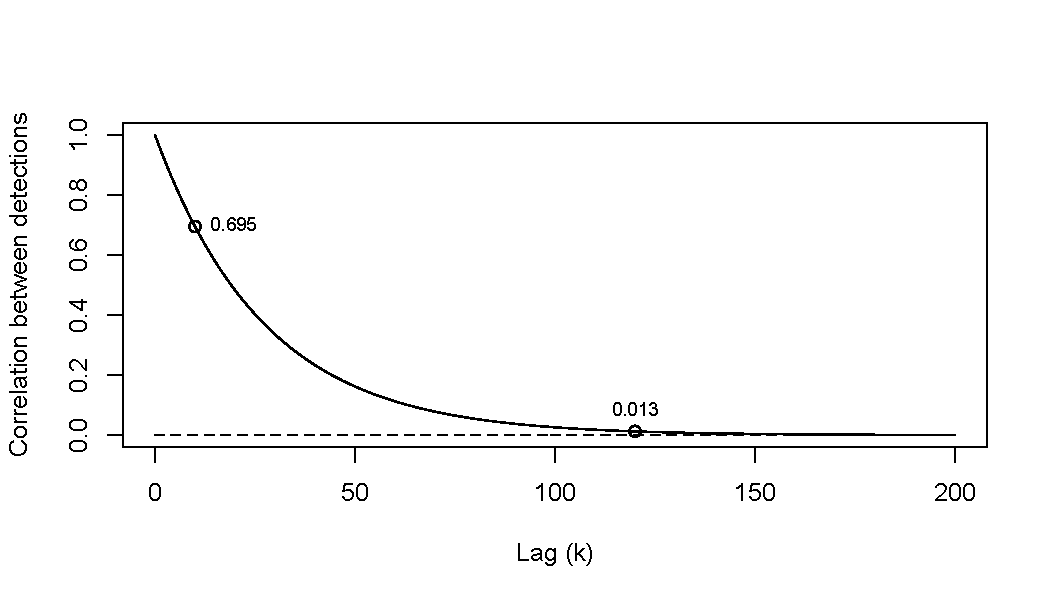
\includegraphics[width=12cm]{HMMcorr.pdf}
\caption{Correlation of detections at various lags ($k$) for an availability process with mean availability cycle length of 138 and mean proportion of time available of 28/138. Correlations at $k=10$ and $k=120$ are shown explicitly.  \label{fig:HMMcorr}}
\end{center}
\end{figure}

\section{Discussion\label{sec:discussion}}

\begin{itemize}

\item With known capture histories this is a kind of SCR transect search with a continuous time movement model and an availability model. Would improve it if extend theory to include 2D observed locations.

\item If know capture histories, can estimate movement and dive cycle parameters.

\item Add covariates to any of the models

\item Slower moving observers: need to take account of first passage time (which ccr method does not).

\item Add more dive states, e.g. split ``near-surface'' state into ``breaking surface'' and ``near-surface''. Probably infeasible as this adds another 4 parameters. Probably only feasible with known capture histories.

\end{itemize}



\appendix
%\appendixpage

\section{Derivation of $f_{T|k}(t|k)$}
\label{appx:firstpassage}

One can view the poblem of finding the pdf of the time between the first and second observers passing an animal as a the problem of finding the first passage time to a point at distance $vk$ from the origin, of a particle following Brownian motion starting at the origin, with constant drift velocity $v$ and diffusion parameter $\sigma$. We can write the process as $Y_t=\sigma B_t+vt$, where $B$ is a Brownian motion and $Y_t$ is the animal's displacement at time $t$. 

\todo[inline]{Currently this is based on these two pages: https://math.stackexchange.com/questions/1053294/density-of-first-hitting-time-of-brownian-motion-with-drift and https://math.stackexchange.com/questions/179210/derivation-of-wiener-process-first-passage-times-using-probability-generating-fu}

From the first of the above sites:

Suppose that $X_t=B_t+ct$, where $B$ is a Brownian motion, $c$ is a constant. Set $H_a=\inf\{t: X_t=a\}$ for $a>0$. It follows that for $c\in\mathbb{R}$, the density of $H_a$ is 
\begin{equation}
f_{H_a} (t) = \frac{ a \exp \Big\{ \frac{- (a-ct)^2}{2t} \Big\} }{\sqrt{2 \pi t^3}}.
\end{equation}

In our case, we have an animal appoaching the ``boundary'' (second observer) that is a distance $vk$ from the starting position of the animal, at speed $v$, and the animal moving according to brownian motion with parameter $\sigma$, so that $Y_t=\sigma B_t+vt$. If we rescale distance to be in units of $\sigma$, i.e. $X_t=Y_t/\sigma$, we have $X_t=B_t+\frac{v}{\sigma}t$ and $a=vk/\sigma$. Hence the pdf of time to the second observer passing, given that the second observer passes a fixed point at a time $k$ later than the first, is
\be
f_{T|k} (t|k)
&=&
\frac{\frac{vk}{\sigma} \exp \Big\{ \frac{- (vk/\sigma-vt/\sigma)^2}{2t} \Big\} }{\sqrt{2 \pi t^3}} 
\;=\;
\frac{vk \exp \Big\{ \frac{- v^2(k-t)^2}{2\sigma^2t} \Big\} }{\sqrt{2 \pi\sigma^2 t^3}}.
\ee




\section{Summary of inputs and outputs\label{appx:notation}}

Evaluation of the above likelihood requires the following inputs:

\begin{itemize}
\item[$\theta_1$:] the density parameter, 
\item[$\theta_2$:] a parameter governing transition from state 1 (surface) to state 2 (underwater),
\item[$\mu_c$:] the expected dive cycle duration,
\item[$p(1)$:] the probability that observer 1 detects an animal that is on the surface,
\item[$p(2)$:] the probability that observer 2 detects an animal that is on the surface,
\item[$\theta_3$:] the log of animal movement speed,
\item[$k$:] the time separation between observers,
\item[$L$:] the total distance flown by the observers,
\item[$s_{11},\ldots,s_{1n_1}$:] the distances along the flight path at which the $n_1$ animals detected by observer 1 were detected, 
\item[$s_{21},\ldots,s_{2n_2}$:] the distances along the flight path at which the $n_2$ animals detected by observer 2 were detected, 
\item[$d_{max}$:] the distance beyond which detections by different observers are certainly detections of different animals,
\item[$\delta_{si}$:] the distance (in observer-seconds) that the $i$th animal moves between the first and second observer passing it,\item[$t_i=k+\delta_{si}$:] the time between first and second observer passing animal $i$.
\end{itemize}

\noindent
from which it should return the value of the likelihood function $\mathcal{L}(k)$.





\bibliographystyle{biom} 
\bibliography{dlb}

\newpage
\section*{Online supplementary material}


\end{document}
